\section{Kalman-Filter \dcsecondauthorshort}
\label{sec:fahrspurerkennung_kalman}

\subsection{Überblick} \label{ssec:fahrspurerkennung:kalman-filter:ueberblick}
Auch der folgende Ansatz zur Fahrspurerkennung approximiert den Verlauf der Fahrspur als Polynom 3. Grades. Jedoch wird nicht mehr jede Fahrspurmarkierung einzeln modelliert, sondern nur noch die Mittellinie. Um die seitlichen Fahrbahnmarkierungen zu erhalten, können beliebige Punkte des Polynoms senkrecht zu dessen Verlauf um die Fahrspurbreite verschoben werden.
Das in \ref{sec:grundlagen:kalman-filter} eingeführte Kalman-Filter soll verwendet werden um die Lage der Fahrbahnmarkierungen in konsekutiven Aufnahmen zu verfolgen. Final sollen Punkte aus den in Einzelbildern erkannten Verläufen der Straßenmarkierung entnommen, in die Weltkarte eingetragen und somit für den Regelungsalgorithmus verfügbar gemacht werden.

\subsection{Fahrspurmodell}
Als Repräsentation der Fahrspur im Zustandsraum soll das in \autocite{petersfalkoFPGAbasierteBildverarbeitungspipelineZur2009} vorgeschlagene Modell, welches wiederum eine Vereinfachung von \autocite{risackRobustLaneRecognition} darstellt, verwendet werden.
Wie in \ref{ssec:fahrspurerkennung:kalman-filter:ueberblick} angekündigt, soll die Fahrspur als Polynom 3. Grades \begin{math} \gls{y}_{\gls{lat:LinienKOS}}(\gls{x}_{\gls{lat:LinienKOS}}) \end{math} approximiert werden. Um die \glsdesc{lat:systemmatrix} \gls{lat:systemmatrix} zu vereinfachen und einen sehr anschaulichen \glsdesc{lat:statevector} \gls{lat:statevector} zu erhalten, wird für jenen die 0. bis 3. Ableitung des Polynoms an der Stelle \begin{math} \gls{x}_{\gls{lat:LinienKOS}}=0 \end{math} verwendet. 
\begin{equation}
\label{eq:polylane}
\gls{y}(\gls{x}) =
\scl{a} +
\scl{b} \cdot \gls{x} +
\scl{c} \cdot \gls{x}^2 +
\scl{d} \cdot \gls{x}^3
\end{equation}
\begin{equation}
\label{eq:statevectorlane}
\gls{lat:statevector} = 
\begin{pmatrix}
\gls{y}_{\gls{lat:LinienKOS}}(0) \\
\der{\gls{y}_{\gls{lat:LinienKOS}}}(0) \\
\derII{\gls{y}_{\gls{lat:LinienKOS}}}(0) \\
\derIII{\gls{y}_{\gls{lat:LinienKOS}}}(0) \\
\end{pmatrix}
=
\begin{pmatrix}
\scl{a} \\
\scl{b} \\
2 \cdot \scl{c} \\
6 \cdot \scl{d} \\
\end{pmatrix}
=
\begin{pmatrix}
\gls{lat:lateraloffset} \\
\gls{gre:yawangle} \\
\gls{lat:curvature} \\
\gls{lat:curvaturechange} \\
\end{pmatrix}
\end{equation}
\begin{equation}
\label{eq:polylanestate}
\gls{y}_{\gls{lat:LinienKOS}}(\gls{x}_{\gls{lat:LinienKOS}}) =
\gls{lat:lateraloffset} +
\gls{gre:yawangle} \cdot \gls{x}_{\gls{lat:LinienKOS}} +
\frac{1}{2} \cdot \gls{lat:curvature} \cdot \gls{x}_{\gls{lat:LinienKOS}}^2 +
\frac{1}{6} \cdot \gls{lat:curvaturechange} \cdot \gls{x}_{\gls{lat:LinienKOS}}^3
\end{equation}
 
\subsubsection{Initialisierung} 
\label{sssec:fahrspurerkennung:kalman:fahrspurmodell:initialisierung}
 Die Initialisierung des Fahrspurmodells erfolgt durch das Finden der Mittellinie auf dem unmaskierten Bild wie in \ref{par:maskenbau:initial} oder mittels des Riverflow-Algorithmus für die mittlere Fahrbahnmarkierung, beschrieben in \ref{ssec:fahrspurerkennung:riverflow:mittellinie}.
 
 \begin{figure}[htb]
 	\centering
 	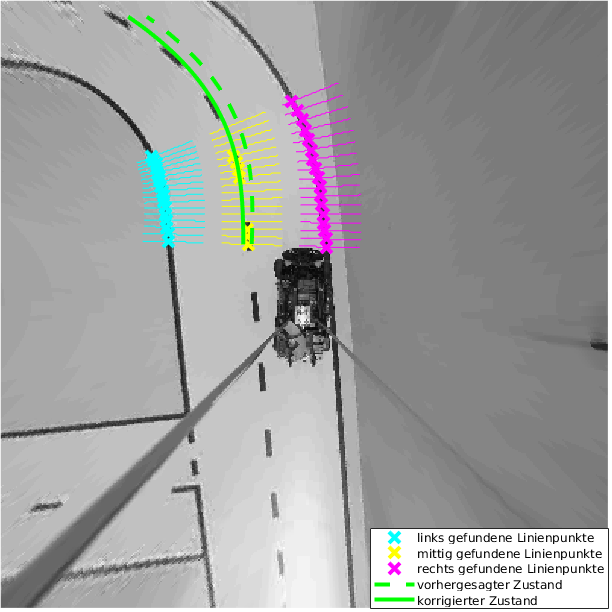
\includegraphics[width=0.75\textwidth]{kalman_iteration_komplett}
 	\caption{Plot einer Iteration des Kalmanfilters}
 	\label{fig:kalman:iteration_komplett}
 \end{figure}
 
\subsection{Messung} \label{ssec:fahrspurerkennung:kalman:messung}
Um eine ausreichende Geschwindigkeit des Kalmanfilters zu gewährleisten, muss die Anzahl der Bildpunkte, welche zur Korrektur des prädizierten Zustands verwendet werden, im Gegensatz zu \ref{sec:maskenbau} vermindert werden. Es wird in Anlehnung an \autocite{risackRobustLaneRecognition} das Bild ab dem Vorverarbeitungsschritt nur in relevanten Bereichen betrachtet.
Hierfür werden Geraden \glqq Scanlines\grqq{} senkrecht zum Polynom des Fahrspurmodells berechnet. Deren Länge sowie Abstand der Startpunkte auf dem Polynom sind als Parameter anzusehen. Nun werden die Helligkeitswerte der Bildpunkte, durch welche die Gerade verläuft, mit dem aus \ref{sec:bildvorverarbeitung:filterung} bekannten Kantendetektor gefiltert. Die Koordinaten der ausreichend großen lokalen Maxima der Filterantwort sind Kandidaten für zentral in der mehrere Pixel breiten mittleren Fahrbahnmarkierung gelegenen Punkte.

\subsubsection{Randlinen}
Um auch die zentral in der äußeren Fahrbahnmarkierung liegenden Punkte detektieren zu können, werden die Scanlines der Mittelline um die Fahrspurbreite senkrecht zum Polynom verschoben. Nun kann derselbe Algorithmus wie für die Scanlines der mittleren Fahrbahnmarkierung ausgeführt werden. Die gefundenen Koordinaten müssen letztendlich wieder um die Fahrspurbreite zur Mittellinie hin verschoben werden um problemlos zur Zustandskorrektur des Kalmanfilters nutzbar zu sein.
 
\subsection{Zustandsraumbeschreibung}
Da die Herleitung der diskreten Zustandsraumbeschreibung zum aufgestellten Fahrspurmodell einfacher ist als der Umweg über eine Kontinuierliche, wird dieser Ansatz nun verfolgt.
Die \glsdesc{lat:systemmatrix} \gls{lat:systemmatrix} bildet den momentanen \glsdesc{lat:statevector} \(\gls{lat:statevector}(\scl{k})\) auf den folgenden \glsdesc{lat:statevector} \(\gls{lat:statevector}(\scl{k}+1)\) ab, ohne äußere Einflüsse auf das System zu berücksichtigen. Die Lage der Fahrbahnmarkierungen im nächsten Bild soll also auf Basis des aktuellen Bildes vorhergesagt werden.

\subsubsection{Vereinfachungen}
Der Einfluss des Lenkwinkels wird vernachlässigt, da er bei kurzer Periodendauer der Abtastung \(\scl{T_s} = \frac{1}{\text{Bildrate}}\)\scl{T_s} und kleiner Größe seiner selbst kaum Einfluss auf die Lage der Fahrbahn im Folgebild nimmt. Die Bewegung des Fahrzeugs wird also geradlinig in Richtung der Abszisse des Fahrspurkoordinatensystems \gls{lat:LinienKOS} angenommen. 

\subsubsection{Herleitung der Systemmatrix}
Der zurückgelegte Weg \begin{math} \scl{\Delta\gls{x}}_{\gls{lat:LinienKOS}} \end{math} zwischen zwei Bildaufnahmenpunkten kann direkt aus den Encodern des Fahrzeugs ausgelesen werden. Der Folgezustand  \(\gls{lat:statevector}(\scl{k}+1)\) wird wie folgt berechnet:
\begin{equation}
\label{eq:nextstatemapping}
\hat{\gls{lat:statevector}}(\scl{k}+1) =
\begin{pmatrix}
\gls{y}_{\gls{lat:LinienKOS}\scl{k}}(\scl{\Delta\gls{x}}_{\gls{lat:LinienKOS}}) \\
\der{\gls{y}_{\gls{lat:LinienKOS}\scl{k}}}(\scl{\Delta\gls{x}}_{\gls{lat:LinienKOS}}) \\
\derII{\gls{y}_{\gls{lat:LinienKOS}\scl{k}}}(\scl{\Delta\gls{x}}_{\gls{lat:LinienKOS}}) \\
\derIII{\gls{y}_{\gls{lat:LinienKOS}\scl{k}}}(\scl{\Delta\gls{x}}_{\gls{lat:LinienKOS}}) \\
\end{pmatrix}
\end{equation}

In \autocite{petersfalkoFPGAbasierteBildverarbeitungspipelineZur2009} wird beschrieben, dass sich aufgrund von Nichtlinearität aus \ref{eq:nextstatemapping} keine äquivalente Matrix A aufstellen lässt. Da diese Nichtlinearität jedoch nur in Bezug auf \scl{\Delta\gls{x}} und nicht den \glsdesc{lat:statevector} \gls{lat:statevector} besteht, ist dies trotz dessen möglich. Aus \eqref{eq:polylanestate}, \eqref{eq:nextstatemapping} und der Bewegung des Fahrzeugs entlang der x-Achse des Fahrspurkoordinatensystems \gls{lat:LinienKOS} um \scl{\Delta\gls{x}} folgt:
\begin{equation}
\begin{split}
\label{eq:nextstatemappingmatrix}
\hat{\gls{lat:statevector}}(\scl{k}+1) = &
\begin{pmatrix}
\gls{lat:lateraloffset} +
\gls{gre:yawangle} \cdot \scl{\Delta\gls{x}} +
\frac{1}{2} \cdot \gls{lat:curvature} \cdot (\scl{\Delta\gls{x}})^2 +
\frac{1}{6} \cdot \gls{lat:curvaturechange} \cdot (\scl{\Delta\gls{x}})^3 \\
\gls{gre:yawangle} + \gls{lat:curvature} \cdot \scl{\Delta\gls{x}} +
\frac{1}{2} \cdot \gls{lat:curvaturechange} \cdot (\scl{\Delta\gls{x}})^2 \\
\gls{lat:curvature} + \gls{lat:curvaturechange} \cdot \scl{\Delta\gls{x}} \\
\gls{lat:curvaturechange}
\end{pmatrix} \\
& \begin{pmatrix}
1 &  \scl{\Delta\gls{x}} & \frac{1}{2} \cdot (\scl{\Delta\gls{x}})^2 & 
\frac{1}{6} \cdot (\scl{\Delta\gls{x}})^3 \\
0 & 1 &  \scl{\Delta\gls{x}} & \frac{1}{2} \cdot (\scl{\Delta\gls{x}})^2 \\
0 & 0 & 1 &  \scl{\Delta\gls{x}} \\
0 & 0 & 0 & 1
\end{pmatrix}
\cdot
\begin{pmatrix}
\gls{lat:lateraloffset} \\
\gls{gre:yawangle} \\
\gls{lat:curvature} \\
\gls{lat:curvaturechange} \\
\end{pmatrix} \\
& \gls{lat:systemmatrix}
\cdot
\begin{pmatrix}
\gls{lat:lateraloffset} \\
\gls{gre:yawangle} \\
\gls{lat:curvature} \\
\gls{lat:curvaturechange} \\
\end{pmatrix}
\end{split}
\end{equation}

Die in \autocite{petersfalkoFPGAbasierteBildverarbeitungspipelineZur2009} durch Linearisierung an der Stelle \begin{math} \gls{x}_{\gls{lat:LinienKOS}0} = 0 \end{math} erhaltene Matrix hingegen vereinfacht sich durch \eqref{eq:generallinearization} zu:

\begin{equation}
\label{eq:nextstatemappingmatrixlinear}
\hat{\gls{lat:statevector}}(\scl{k}+1) =
\begin{pmatrix}
\gls{lat:lateraloffset} + \gls{gre:yawangle} \cdot \scl{\Delta\gls{x}} \\
\gls{gre:yawangle} + \gls{lat:curvature} \cdot \scl{\Delta\gls{x}}\\
\gls{lat:curvature} + \gls{lat:curvaturechange} \scl{\Delta\gls{x}} \\
\gls{lat:curvaturechange}
\end{pmatrix}
=
\begin{pmatrix}
1 &  \scl{\Delta\gls{x}} & 0 & 0 \\
0 & 1 &  \scl{\Delta\gls{x}} & 0 \\
0 & 0 & 1 &  \scl{\Delta\gls{x}} \\
0 & 0 & 0 & 1
\end{pmatrix}
\cdot
\begin{pmatrix}
\gls{lat:lateraloffset} \\
\gls{gre:yawangle} \\
\gls{lat:curvature} \\
\gls{lat:curvaturechange} \\
\end{pmatrix}
=
\gls{lat:systemmatrix}
\cdot
\begin{pmatrix}
\gls{lat:lateraloffset} \\
\gls{gre:yawangle} \\
\gls{lat:curvature} \\
\gls{lat:curvaturechange} \\
\end{pmatrix}
\end{equation}

\begin{equation}
\label{eq:generallinearization}
\fnf{\gls{x}_{\gls{lat:LinienKOS}}} \approx \fnf{\gls{x}_{\gls{lat:LinienKOS}0}} + 
%\frac{df}{d\gls{x}}|_{\gls{x}_0} \cdot
\derat{\fnfop}{\gls{x}_{\gls{lat:LinienKOS}0}} \cdot
(\gls{x}-\gls{x}_0)
\end{equation}

Da sich die gefahrene Strecke \begin{math} \scl{\Delta\gls{x}}_{\gls{lat:LinienKOS}} \end{math} zwischen den Aufnahmepunkten zweier Bilder geringfügig ändern kann, muss die \glsdesc{lat:systemmatrix} \gls{lat:systemmatrix} vor jedem Prädikationsschritt neu berechnet werden.

\subsubsection{Eingangsmatrix}
Die \glsdesc{lat:inputmatrix} \gls{lat:inputmatrix} modelliert äußere Einflüsse auf die Entwicklung des Systemzustandes \gls{lat:statevector}. Dies könnten z.B. Änderungen des Lenkwinkels sein. Da letzterer jedoch schon bei der Herleitung der \glsdesc{lat:systemmatrix} \gls{lat:systemmatrix} vernachlässigt wurde, kann \gls{lat:inputmatrix} bei weiteren Untersuchungen unberücksichtigt bleiben.

\subsubsection{Ausgangsmatrix/Messmatrix} 
\label{sssec:fahrspurerkennung:kalman-filter:zustandsraumbeschreibung:outputmatrix}
Die \glsdesc{lat:outputmatrix} \gls{lat:outputmatrix} bildet den Systemzustand \gls{lat:statevector} auf eine Messung \gls{lat:outputvector} ab. In unserer Implementierung wird  \gls{lat:outputmatrix} passend zu den \gls{x}-Koordinaten der wie in \ref{ssec:fahrspurerkennung:kalman:messung} beschrieben gewonnenen Linienmittelpunkte in jeder Iteration des Kalmanfilters neu berechnet. Aus \ref{eq:polylanestate} ergibt sich:
\begin{equation}
\begin{split}
\gls{lat:outputvector} & =
\begin{pmatrix}
\gls{y}_{\gls{lat:LinienKOS}1} \\
\gls{y}_{\gls{lat:LinienKOS}2} \\
\vdots \\
\gls{y}_{\gls{lat:LinienKOS}\scl{n}}
\end{pmatrix}
=
\begin{pmatrix}
\gls{lat:lateraloffset} +
\gls{gre:yawangle} \cdot \gls{x}_{\gls{lat:LinienKOS}1} +
\frac{1}{2} \cdot \gls{lat:curvature} \cdot \gls{x}_{\gls{lat:LinienKOS}1}^2 +
\frac{1}{6} \cdot \gls{lat:curvaturechange} \cdot \gls{x}_{\gls{lat:LinienKOS}1}^3  \\
\gls{lat:lateraloffset} +
\gls{gre:yawangle} \cdot \gls{x}_{\gls{lat:LinienKOS}2} +
\frac{1}{2} \cdot \gls{lat:curvature} \cdot \gls{x}_{\gls{lat:LinienKOS}2}^2 +
\frac{1}{6} \cdot \gls{lat:curvaturechange} \cdot \gls{x}_{\gls{lat:LinienKOS}2}^3  \\
\vdots \\
\gls{lat:lateraloffset} +
\gls{gre:yawangle} \cdot \gls{x}_{\gls{lat:LinienKOS}\scl{n}} +
\frac{1}{2} \cdot \gls{lat:curvature} \cdot \gls{x}_{\gls{lat:LinienKOS}\scl{n}}^2 +
\frac{1}{6} \cdot \gls{lat:curvaturechange} \cdot 
\gls{x}_{\gls{lat:LinienKOS}\scl{n}}^3  
\end{pmatrix} \\
& =
\begin{pmatrix}
1 & \gls{x}_{\gls{lat:LinienKOS}1} & \frac{1}{2} \cdot \gls{x}_{\gls{lat:LinienKOS}1}^2 &
\frac{1}{6} \cdot \gls{x}_{\gls{lat:LinienKOS}1}^3  \\
1 & \gls{x}_{\gls{lat:LinienKOS}2} & \frac{1}{2} \cdot \gls{x}_{\gls{lat:LinienKOS}2}^2 &
\frac{1}{6} \cdot \gls{x}_{\gls{lat:LinienKOS}2}^3  \\
\vdots & \vdots & \vdots & \vdots \\
1 & \gls{x}_{\gls{lat:LinienKOS}\scl{n}} & 
\frac{1}{2} \cdot \gls{x}_{\gls{lat:LinienKOS}\scl{n}}^2 &
\frac{1}{6} \cdot \gls{x}_{\gls{lat:LinienKOS}\scl{n}}^3
\end{pmatrix}
\cdot
\begin{pmatrix}
\gls{lat:lateraloffset} \\
\gls{gre:yawangle} \\
\gls{lat:curvature} \\
\gls{lat:curvaturechange} \\
\end{pmatrix}
\end{split}
\end{equation} 

\subsection{Kovarianzmatritzen}
Wie in \autocite{petersfalkoFPGAbasierteBildverarbeitungspipelineZur2009} und \autocite{risackRobustLaneRecognition} werden die Kovarianzmatrix des System-/Prozessrauschens \mtx{Q} und die Kovarianzmatrix des Messrauschens \mtx{R} als konstante Diagonalmatritzen gesetzt. Auf die Prädiktion der Kovarianzmatrix \mtx{P} wird somit verzichtet.

\subsection{konkrete Implementierung des Kalman-Filters}
Ist der \glsdesc{lat:statevector} \gls{lat:statevector} einmal wie in ~\ref{sssec:fahrspurerkennung:kalman:fahrspurmodell:initialisierung} beschrieben initialisiert, können die Gleichungen des Kalmanfilters bei Eintreffen eines neuen Bildes wie folgt berechnet werden:
\begin{enumerate}
\item Bildung der \glsdesc{lat:systemmatrix} \gls{lat:systemmatrix} mittels der seit dem letzten Bild gefahrenen Distanz \scl{\Delta\gls{x}}
\item Prädiktion des \glsdesc{lat:statevector} \gls{lat:statevector}, d.h. der Lage der Fahrspurmarkierungen im aktuellen Bild anhand von \eqref{eq:kalmanprediction}
\item Messung der Lage der Fahrspur wie in \ref{ssec:fahrspurerkennung:kalman:messung}
erläutert
\item Bildung der \glsdesc{lat:outputmatrix} \gls{lat:outputmatrix} passend zur Messung wie in \ref{sssec:fahrspurerkennung:kalman-filter:zustandsraumbeschreibung:outputmatrix} beschrieben
\item Korrektur des \glsdesc{lat:statevector}s \gls{lat:statevector} unter Nutzung von \eqref{eq:kalmancorrection}
\end{enumerate}




